\documentclass{article}
\usepackage[headheight=40pt, textheight=560pt]{geometry}
\usepackage{paralist}
\usepackage{scalerel,amssymb}
\usepackage{amsmath}
\usepackage{colortbl}
\usepackage{array}
\usepackage{multirow}
\usepackage{blindtext}
\usepackage{reledmac}
\usepackage{changepage}

\usepackage{pgfplots}
\usepackage{tikz}
\usetikzlibrary{positioning}
\usetikzlibrary{shapes.geometric, arrows}
\tikzstyle{arrow} = [thick,->,>=stealth]

\usepackage{graphicx}
\usepackage{stix}

\newcommand{\tableflip}{$($\rotatebox{45}{$\smile$}$^{\circ}\smwhtsquare^{\circ})\rotatebox{45}{$\smile$}\mkern-6mu\frown$\raisebox{0.5ex}{$\bot$}$\mkern-3.5mu-\mkern-3.5mu$\raisebox{0.5ex}{$\bot$}}

\usepackage{stackengine}
\def\apeqA{\SavedStyle\sim}
\def\apeq{\setstackgap{L}{\dimexpr.5pt+1.5\LMpt}\ensurestackMath{%
  \ThisStyle{\mathrel{\Centerstack{{\apeqA} {\apeqA} {\apeqA}}}}}}

\usepackage{fancyhdr}
\fancyhead[L]{
	\begin{tabular}{ll}
		\begin{tabular}{l}
			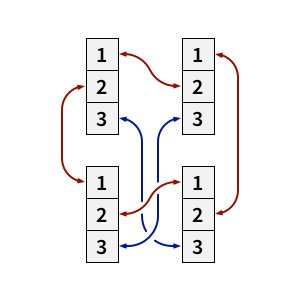
\includegraphics[scale=0.13]{distributed}
		\end{tabular}	
		&
		\begin{tabular}{l}
			\LARGE \textbf{Distributed Algorithms} \\
			\Large \textsc{Lectures}
		\end{tabular}
	\end{tabular}
}
\fancyhead[R]{
	\begin{tabular}{r}
		16-124-836 \\
		Marcel \textsc{Zauder}
	\end{tabular}
}
\renewcommand{\headrulewidth}{0.4pt}
\fancyfoot[C]{\thepage}
\renewcommand{\footrulewidth}{0.4pt}

\usepackage{hyperref}

\begin{document}
	\pagestyle{fancy}
	\section{Introduction - February 19, 2020}
	\begin{adjustwidth}{2em}{2em}
		\subsection{Defining Dependable Systems}
		\begin{adjustwidth}{2em}{2em}
			\textsc{Quotes:}
			\begin{adjustwidth}{2em}{}
				\textit{A distributed system is a system where a computer of which you did not know it exists can prevent you from getiing your job done.} - Leslie \textsc{Lamport}
			\end{adjustwidth}
			\vspace{0.2cm}
			\begin{adjustwidth}{2em}{}
				\textit{There is perhaps a market for maybe five computers in the world.} - TJ \textsc{Watson}
			\end{adjustwidth}
			\hfill \\
			\textsc{Fault} $\rightarrow$ \textsc{Error} $\rightarrow$ \textsc{Failure}
			\begin{compactenum}[-]
				\item Train delayed because of tree has fallen on the tracks
				\item Travelers reach destination too late
				\item Alice misses her exam
			\end{compactenum}
			\vspace{0.2cm}
			\begin{tabular}{|l|lll|}
				\hline
				& \underline{\textsc{Fault}} & \underline{\textsc{Error}} & \underline{\textsc{Failure}} \\
				\hline
				Train: & Tree fallen & no train & delay for passengers \\
				Journey: & Train delay & delay & reached destination 2h after intention \\
				Exam: & arrival 2h late & missed time-slot & repeat exam \\
				\hline
			\end{tabular}
			\hfill \\
			\underline{\textsc{Fault:}} cause of failure \\
			\underline{\textsc{Error:}} internal state of system, not according to specification \\
			\underline{\textsc{Failure:}} observable deviation of specification
			\hfill \\ \\
			\underline{\textsc{Fault} examples:}
			\begin{compactenum}[-]
				\item timing
				\item cables
				\item power supply
				\item messages lost
				\item data loss (solved with RAIDs)
			\end{compactenum}
			\subsubsection{\underline{How to make systems tolerate faults}}
			\begin{adjustwidth}{2em}{}
				\begin{compactenum}[-]
					\item \textsc{Prevention}
					\item \textsc{Tolerance}
					\begin{compactenum}[\textbullet]
						\item Replication/Redundancy
						\item Recovery
					\end{compactenum}
					\item \textsc{Removal}
					\item \textsc{Forecasting/Prediction}
				\end{compactenum}
			\end{adjustwidth}
			\hfill \\
			\textsc{Safety} $\neq$ \textsc{Security} \\
			\textsc{Safety} is connected to loss of live/material due to accidents \\
			\textsc{Security} is connected to malicious intent
			\subsubsection{Defining distributed computation}
			\begin{adjustwidth}{2em}{}
				Processes $\Pi = \{ p,q,r,s \ldots \}$ \\
				$\mid \Pi \mid = N$
				
				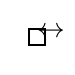
\begin{tikzpicture}[-,thick,every node/.style={shape=rectangle,inner sep=3pt,draw,thick}]
					p			q			....	s
  					\node{};	\node{};			\node{};
  					\node{};	\node{};			\node{};
  					\node{};	\node{};			\node{};
  					BUS $\leftrightarrow$
				\end{tikzpicture}
				\hfill \\
				\underline{\textsc{Components}} \\
				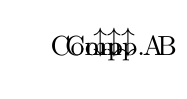
\begin{tikzpicture}
					$\updownarrow$
					\node{Comp. A};
					$\updownarrow$
					\node{Comp. B};
					$\updownarrow$
				\end{tikzpicture}
				\hfill \\
				\textsc{Events} for Component $c$:
				\[
					\langle c, event \mid param_1 , param_2 \ldots \rangle
				\]
				\underline{upon} $\langle c, ev_1 \mid param_1 \rangle$ \underline{do}
				\begin{adjustwidth}{1em}{}
					do something \\
					\underline{trigger} $\langle \textit{b, domore} \mid p \rangle$
				\end{adjustwidth}
				\hfill \\
				\underline{upon} $\langle \textit{b, domore} \mid p \rangle$ \underline{do}
			\end{adjustwidth}
			\subsubsection{Layered modules}
			\begin{adjustwidth}{2em}{}
				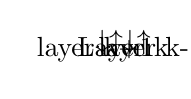
\begin{tikzpicture}
					\node{layer k+1};
					$\downarrow$(blue) "send" || $\uparrow$(red) "deliver"
					\node{Layer k};
					invoke || receive
					$\downarrow$(blue) "unreliable send" || $\uparrow$(red) "unreliable deliver"
					\node{layer k-1};
				\end{tikzpicture}
				\hfill \\
				Events either travel:
				\begin{compactenum}[-]
					\item upwards (red): indication
					\item downwards (blue): request
				\end{compactenum}
				\vspace{0.3cm}
				Events on a given layer may be:
				\begin{compactenum}[-]
					\item input events (IN)
					\item output events (OUT)
				\end{compactenum}
			\end{adjustwidth}
			\subsubsection{Module Jobhandler}
			\begin{adjustwidth}{2em}{}
				\underline{Events:}
				\begin{adjustwidth}{1em}{}
					Request: $\langle \textit{jh, handle} \mid \textit{job} \rangle$ \\
					Indication: $\langle \textit{jh, confirm} \mid \textit{job} \rangle$
				\end{adjustwidth}
				\underline{Properties:}
				\begin{adjustwidth}{1em}{}
					Every job submitted for handling is eventually confirmed.
				\end{adjustwidth}
				\hfill \\
				\underline{Implementation (synchronized)} \textsc{JobHandler} \\
				\underline{State}
				\begin{adjustwidth}{1em}{}
					\ldots
				\end{adjustwidth}
				\underline{upon} $\langle \textit{jh, handle} \mid \textit{job} \rangle$ \underline{do}
				\begin{adjustwidth}{1em}{}
					"process job" \\
					\underline{trigger} $\langle \textit{jh, confirm} \mid \textit{job} \rangle$
				\end{adjustwidth}
				\vspace{0.2cm}
				\underline{upon} \ldots \\
				\underline{upon} \ldots \\ \\
				\underline{Implementation (asynchronized)} \textsc{JobHandler} \\
				\underline{State}
				\begin{adjustwidth}{1em}{}
					\textit{buf} $\leftarrow \emptyset$
				\end{adjustwidth}
				\underline{upon} $\langle \textit{jh, handle} \mid \textit{job} \rangle$ \underline{do}
				\begin{adjustwidth}{1em}{}
					\textit{buf} $\leftarrow$ \textit{buf} $\cup \{ \textit{job} \}$ \\
					\underline{trigger} $\langle \textit{jh, confirm} \mid \textit{job} \rangle$
				\end{adjustwidth}
				\vspace{0.2cm}
				\underline{upon} \textit{buf} $\neq \emptyset$ \underline{do}
				\begin{adjustwidth}{1em}{}
					\textit{job} $\leftarrow$ some element of \textit{buf} \\
					"process job" \\
					\textit{buf} $\leftarrow$ \textit{buf} $\setminus \{ \textit{job} \}$
				\end{adjustwidth}
			\end{adjustwidth}
		\end{adjustwidth}
		\subsection{Concurrency and Replication in Distributed Systems}
		\begin{adjustwidth}{2em}{2em}
		\end{adjustwidth}
	\end{adjustwidth}
	
	\newpage
	
	\section{2nd Lecture - \today}
	\begin{adjustwidth}{2em}{2em}
	\end{adjustwidth}
\end{document}